%!Tex Root = ../Main.tex
% ./Packete_und_Deklarationen.tex
% ./Titlepage.tex
% ./Motivation.tex
% ./Einführung.tex
% ./Ergebnisse_und_Ausblick.tex

\chapter{Implementierung}
\label{ch:implementierung}
\section{Architektur}
% Unterscheid zur Architektur aus dem Bachelorprojekt

% Cross Compiler
\begin{figure}
  \centering
  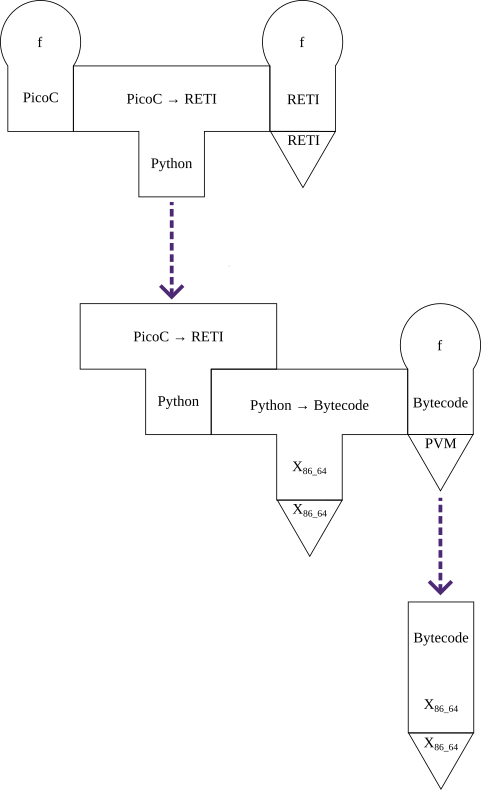
\includegraphics[width=0.5\linewidth]{./figures/summarized_cross_compiler.png}
  \caption{Cross-Compiler Kompiliervorgang ausgeschrieben}
\end{figure}

\begin{figure}
  \centering
  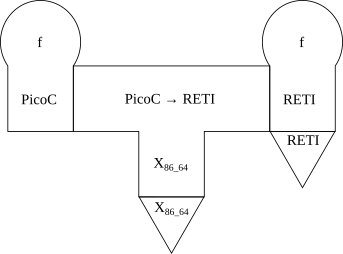
\includegraphics[width=0.33\linewidth]{./figures/compiliervorang_mit_machiene.png}
  \caption{Cross-Compiler Kompiliervorgang Kurzform}
\end{figure}

\begin{figure}
  \centering
  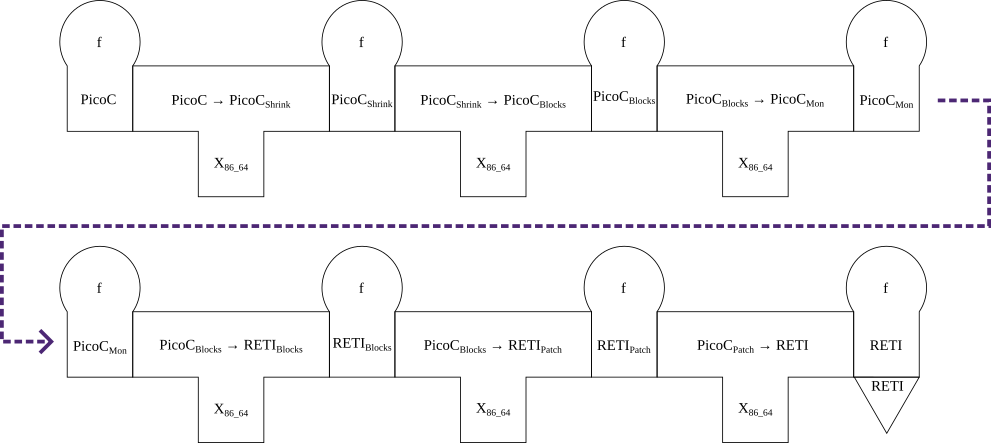
\includegraphics[width=\linewidth]{./figures/passes.png}
  \caption{Architektur mit allen Passes ausgeschrieben}
\end{figure}

\section{Lexikalische Analyse}
\subsection{Verwendung von Lark}
% erwähnen, dass in Lark die Grammatiken L_Lex und L_Parse gemischt sind
% EBNF erwähnen
% (erwähnen, dass finalle Grammatik im Appendix)
\subsection{Basic Parser}
\section{Syntaktische Analyse}
\subsection{Verwendung von Lark}
% Vorteile von Lark
\subsection{Umsetzung von Präzidenz}
Die \colorbold{PicoC Sprache} hat dieselben \colorbold{Präzidenzregeln} implementiert, wie die \colorbold{Sprache C} \footcite{noauthor_c_nodate}. Die \colorbold{Präzidenzregeln} von \colorbold{PicoC} sind in Tabelle~\ref{tab:reference_table} aufgelistet.

\begin{table}[H]
  \center
  \begin{tabulary}{\linewidth}{|C|C|L|L|}
  \toprule
  \colorbold{Präzidenz} &	\colorbold{Operator} & \colorbold{Beschreibung} &	\colorbold{Assoziativität} \\
  \midrule
  1	& \verb|a()|	& Funktionsaufruf & \multirow{2}{=}{Links, dann rechts $\rightarrow$} \\
    & \verb|a[]|	& Indexzugriff & \\
    & \verb|a.b| & Attributzugriff & \\
  \hline
  2	&	\verb|-a| & Unäres Minus & \multirow{2}{=}{Rechts, dann links $\leftarrow$} \\
    & \smalltt{!a $\thicksim$a}	& Logisches NOT und Bitweise NOT & \\
    & \verb|*a &a| & Dereferenz und Referenz, auch Adresse-von & \\
  \hline
  3	& \smalltt{a*b a/b a\%b} &	Multiplikation, Division und Modulo & Links, dann rechts $\rightarrow$ \\
  \cline{1-3}
  4	& \verb|a+b a-b|	& Addition und Subtraktion & \\
  \cline{1-3}
  5	& \verb|a<b a<=b| \verb|a>b a>=b| & Kleiner, Kleiner Gleich, Größer, Größer gleich & \\
  \cline{1-3}
  6 &	\verb|a==b a!=b| & Gleichheit und Ungleichheit & \\
  \cline{1-3}
  7 &	\verb|a&b| & Bitweise UND & \\
  \cline{1-3}
  8 &	\verb|a^b| & Bitweise XOR (exclusive or) & \\
  \cline{1-3}
  9 & \smalltt{a$\mid$b} & Bitweise ODER (inclusive or) & \\
  \cline{1-3}
  10	& \verb|a&&b| &	Logiches UND & \\
  \cline{1-3}
  11	& $a{\mid\mid} b$	& Logisches ODER & \\
  \hline
  12 & \verb|a=b| & Zuweisung & Rechts, dann links $\leftarrow$ \\
  \hline
  13 &	\verb|a,b|& Komma	& Links, dann rechts $\rightarrow$ \\
  \bottomrule
\end{tabulary}
\caption{Präzidenzregeln von PicoC}
\label{tab:reference_table}
\end{table}
% erwähnen von Mehrdeutigkeit und Assoziativität
% finalle Grammatik im Appendix
% Crafting Compilers Quelle benennen
\subsection{Derivation Tree Generierung}
\subsection{Early Parser}
\subsection{Derivation Tree Vereinfachung}
% Visitor erwähnen
\subsection{Abstrakt Syntax Tree Generierung}
\subsubsection{ASTNode}
\subsubsection{PicoC Nodes}
% Tabelle aller PicoC Nodes
% möglichst kurze und leicht verständliche Bezeichner für Nodes
\subsubsection{RETI Nodes}
% Tabelle aller RETI Nodes
% Transformer erwähnen
\section{Code Generierung}
\subsection{Passes}
\subsubsection{PicoC-Shrink Pass}
% dieser Pass wurde wegen
\subsubsection{PicoC-Blocks Pass}
\subsubsection{PicoC-Mon Pass}
\begin{Definition}{Symboltabelle}{symboltabelle}
\end{Definition}
\subsubsection{RETI-Blocks Pass}
\subsubsection{RETI-Patch Pass}
\subsubsection{RETI Pass}
% TODO: zusammenfassendes Bild

\subsection{Umsetzung von Pointern}
\subsubsection{Referenzierung}
\begin{code}
  \centering
  \numberedcodebox[minted language=c]{./code_examples/example_pntr_ref.picoc}
  \caption{PicoC Code für Pointer Referenzierung}
  \label{fig:picoc_code_für_pointer_referenzierung}
\end{code}

\begin{code}
  \centering
  \numberedcodebox[minted language=text]{./code_examples/example_pntr_ref.ast}
  \caption{Abstract Syntax Tree für Pointer Referenzierung}
  \label{fig:abstract_syntax_tree_für_pointer_referenzierung}
\end{code}

\begin{code}
  \centering
  \numberedcodebox[minted language=c]{./code_examples/example_pntr_ref.st}
  \caption{Symboltabelle für Pointer Referenzierung}
  \label{fig:symboltabelle_für_pointer_referenzierung}
\end{code}

\begin{code}
  \centering
  \numberedcodebox[minted language=text]{./code_examples/example_pntr_ref.picoc_mon}
  \caption{PicoC Mon Pass für Pointer Referenzierung}
  \label{fig:picoc_mon_für_pointer_referenzierung}
\end{code}

\begin{code}
  \centering
  \numberedcodebox[minted language=text]{./code_examples/example_pntr_ref.reti_blocks}
  \caption{RETI Blocks Pass für Pointer Referenzierung}
  \label{fig:reti_blocks_für_pointer_referenzierung}
\end{code}
% Initialisierung eines Pointers
\subsubsection{Pointer Dereferenzierung durch Zugriff auf Arrayindex ersetzen}
\begin{code}
  \centering
  \numberedcodebox[minted language=c]{./code_examples/example_pntr_deref.picoc}
  \caption{PicoC Code für Pointer Dereferenzierung}
  \label{fig:picoc_code_für_pointer_dereferenzierung}
\end{code}

\begin{code}
  \centering
  \numberedcodebox[minted language=text]{./code_examples/example_pntr_deref.ast}
  \caption{Abstract Syntax Tree für Pointer Dereferenzierung}
  \label{fig:abstract_syntax_tree_für_pointer_dereferenzierung}
\end{code}

\begin{code}
  \centering
  \numberedcodebox[minted language=text]{./code_examples/example_pntr_deref.picoc_shrink}
  \caption{PicoC Shrink Pass für Pointer Dereferenzierung}
  \label{fig:picoc_shrink_für_pointer_dereferenzierung}
\end{code}

\subsection{Umsetzung von Arrays}
\subsubsection{Initialisierung von Arrays}
% Stack und Globale Statische Daten
\begin{code}
  \centering
  \numberedcodebox[minted language=c]{./code_examples/example_array_init.picoc}
  \caption{PicoC Code für Array Initialisierung}
  \label{fig:picoc_code_für_array_initialisierung}
\end{code}

\begin{code}
  \centering
  \numberedcodebox[minted language=text]{./code_examples/example_array_init.ast}
  \caption{Abstract Syntax Tree für Array Initialisierung}
  \label{fig:abstract_syntax_tree_für_array_initialisierung}
\end{code}

\begin{code}
  \centering
  \numberedcodebox[minted language=text]{./code_examples/example_array_init.st}
  \caption{Symboltabelle für Array Initialisierung}
  \label{fig:symboltabelle_für_array_initialisierung}
\end{code}

\begin{code}
  \centering
  \numberedcodebox[minted language=text]{./code_examples/example_array_init.picoc_mon}
  \caption{PicoC Mon Pass für Array Initialisierung}
  \label{fig:picoc_mon_für_array_initialisierung}
\end{code}

\begin{code}
  \centering
  \numberedcodebox[minted language=text]{./code_examples/example_array_init.reti_blocks}
  \caption{RETI Blocks Pass für Array Initialisierung}
  \label{fig:reti_blocks_für_array_initialisierung}
\end{code}


% kleines Extra
\subsubsection{Zugriff auf Arrayindex}

Der Zugriff auf einen bestimmten  Index eines Arrays ist wie folgt umgesetzt:

\begin{code}
  \centering
  \numberedcodebox[minted language=c]{./code_examples/example_array_access.picoc}
  \caption{PicoC Code für Zugriff auf Arrayindex}
  \label{fig:picoc_code_für_zugriff_auf_arrayindex}
\end{code}

\begin{code}
  \centering
  \numberedcodebox[minted language=text]{./code_examples/example_array_access.ast}
  \caption{Abstract Syntax Tree für Zugriff auf Arrayindex}
  \label{fig:abstract_syntax_tree_für_zugriff_auf_arrayindex}
\end{code}

\begin{code}
  \centering
  \numberedcodebox[minted language=text]{./code_examples/example_array_access.picoc_mon}
  \caption{PicoC Mon Pass für Zugriff auf Arrayindex}
  \label{fig:picoc_mon_für_zugriff_auf_arrayindex}
\end{code}

\begin{code}
  \centering
  \numberedcodebox[minted language=text]{./code_examples/example_array_access.reti_blocks}
  \caption{RETI Blocks Pass für Zugriff auf Arrayindex}
  \label{fig:reti_blocks_für_zugriff_auf_arrayindex}
\end{code}

\subsubsection{Zuweisung an Arrayindex}
% Formel aus der Vorlesung, wo ist die hier?
\begin{code}
  \centering
  \numberedcodebox[minted language=c]{./code_examples/example_array_assignment.picoc}
  \caption{PicoC Code für Zuweisung an Arrayindex}
  \label{fig:picoc_code_für_array_assignment}
\end{code}

\begin{code}
  \centering
  \numberedcodebox[minted language=text]{./code_examples/example_array_assignment.ast}
  \caption{Abstract Syntax Tree für Zuweisung an Arrayindex}
  \label{fig:abstract_syntax_tree_für_array_assignment}
\end{code}

\begin{code}
  \centering
  \numberedcodebox[minted language=text]{./code_examples/example_array_assignment.picoc_mon}
  \caption{PicoC Mon Pass für Zuweisung an Arrayindex}
  \label{fig:picoc_mon_für_array_assignment}
\end{code}

\begin{code}
  \centering
  \numberedcodebox[minted language=text]{./code_examples/example_array_assignment.reti_blocks}
  \caption{RETI Blocks Pass für Zuweisung an Arrayindex}
  \label{fig:reti_blocks_für_array_assignment}
\end{code}

\subsection{Umsetzung von Structs}
\subsubsection{Deklaration von Structs}
\begin{code}
  \centering
  \numberedcodebox[minted language=c]{./code_examples/example_struct_decl.picoc}
  \caption{PicoC Code für Deklaration von Structs}
  \label{fig:picoc_code_für_deklaration_von_structs}
\end{code}

\begin{code}
  \centering
  \numberedcodebox[minted language=text]{./code_examples/example_struct_decl.st}
  \caption{Symboltabelle für Deklaration von Structs}
  \label{fig:symboltabelle_für_deklaration_von_structs}
\end{code}

\subsubsection{Initialisierung von Structs}
\begin{code}
  \centering
  \numberedcodebox[minted language=c]{./code_examples/example_struct_init.picoc}
  \caption{PicoC Code für Initialisierung von Structs}
  \label{fig:picoc_code_für_initialisierung_von_structs}
\end{code}

\begin{code}
  \centering
  \numberedcodebox[minted language=text]{./code_examples/example_struct_init.ast}
  \caption{Abstract Syntax Tree für Initialisierung von Structs}
  \label{fig:abstract_syntax_tree_für_initialisierung_von_structs}
\end{code}

\begin{code}
  \centering
  \numberedcodebox[minted language=text]{./code_examples/example_struct_init.st}
  \caption{Symboltabelle für Initialisierung von Structs}
  \label{fig:symboltabelle_für_initialisierung_von_structs}
\end{code}

\begin{code}
  \centering
  \numberedcodebox[minted language=text]{./code_examples/example_struct_init.picoc_mon}
  \caption{PicoC Mon Pass für Initialisierung von Structs}
  \label{fig:picoc_mon_pass_für_initialisierung_von_structs}
\end{code}

\begin{code}
  \centering
  \numberedcodebox[minted language=text]{./code_examples/example_struct_init.reti_blocks}
  \caption{RETI Blocks Pass für Initialisierung von Structs}
  \label{fig:reti_blocks_pass_für_initialisierung_von_structs}
\end{code}

% Stack und Globale Statische Daten
\subsubsection{Zugriff auf Structattribut}
% Formel aus der Vorlesung, wo ist die hier?
\begin{code}
  \centering
  \numberedcodebox[minted language=c]{./code_examples/example_struct_attr_access.picoc}
  \caption{PicoC Code für Zugriff auf Structattribut}
  \label{fig:picoc_code_für_zugriff_auf_structattribut}
\end{code}

\begin{code}
  \centering
  \numberedcodebox[minted language=text]{./code_examples/example_struct_attr_access.ast}
  \caption{Abstract Syntax Tree für Zugriff auf Structattribut}
  \label{fig:abstract_syntax_tree_für_zugriff_auf_structattribut}
\end{code}

\begin{code}
  \centering
  \numberedcodebox[minted language=text]{./code_examples/example_struct_attr_access.picoc_mon}
  \caption{PicoC Mon Pass für Zugriff auf Structattribut}
  \label{fig:picoc_mon_pass_für_zugriff_auf_structattribut}
\end{code}

\begin{code}
  \centering
  \numberedcodebox[minted language=text]{./code_examples/example_struct_attr_access.reti_blocks}
  \caption{RETI Blocks Pass für Zugriff auf Structattribut}
  \label{fig:reti_blocks_pass_für_zugriff_auf_structattribut}
\end{code}

\subsubsection{Zuweisung an Structattribut}
\begin{code}
  \centering
  \numberedcodebox[minted language=c]{./code_examples/example_struct_attr_assignment.picoc}
  \caption{PicoC Code für Zuweisung an Structattribut}
  \label{fig:picoc_code_für_zuweisung_an_structattribut}
\end{code}

\begin{code}
  \centering
  \numberedcodebox[minted language=text]{./code_examples/example_struct_attr_assignment.ast}
  \caption{Abstract Syntax Tree für Zuweisung an Structattribut}
  \label{fig:abstract_syntax_tree_für_zuweisung_an_structattribut}
\end{code}

\begin{code}
  \centering
  \numberedcodebox[minted language=text]{./code_examples/example_struct_attr_assignment.picoc_mon}
  \caption{PicoC Mon Pass für Zuweisung an Structattribut}
  \label{fig:picoc_mon_pass_für_zuweisung_an_structattribut}
\end{code}

\begin{code}
  \centering
  \numberedcodebox[minted language=text]{./code_examples/example_struct_attr_assignment.reti_blocks}
  \caption{RETI Blocks Pass für Zuweisung an Structattribut}
  \label{fig:reti_blocks_pass_für_zuweisung_an_structattribut}
\end{code}

\subsection{Umsetzung der Derived Datatypes im Zusammenspiel}
\subsubsection{Einleitungsteil für Globale Statische Daten und Stackframe}
% Stack und Globale Statische Daten, unterschieldihe Berechnung der Adressen
% unterschiedliche Adressberechnung
\begin{code}
  \centering
  \numberedcodebox[minted language=c]{./code_examples/example_derived_dts_introduction_part.picoc}
  \caption{PicoC Code für den Einleitungsteil}
  \label{fig:picoc_code_einleitungsteil}
\end{code}

% spezielles Vorgehen bei PntrDecl

\begin{code}
  \centering
  \numberedcodebox[minted language=text]{./code_examples/example_derived_dts_introduction_part.ast}
  \caption{Abstract Syntax Tree für den Einleitungsteil}
  \label{fig:abstract_syntax_tree_einleitungsteil}
\end{code}

\begin{code}
  \centering
  \numberedcodebox[minted language=text]{./code_examples/example_derived_dts_introduction_part.picoc_mon}
  \caption{PicoC Mon Pass für den Einleitungsteil}
  \label{fig:picoc_mon_pass_einleitungsteil}
\end{code}

\begin{code}
  \centering
  \numberedcodebox[minted language=text]{./code_examples/example_derived_dts_introduction_part.reti_blocks}
  \caption{RETI Blocks Pass für den Einleitungsteil}
  \label{fig:reti_blocks_pass_einleitungsteil}
\end{code}

\subsubsection{Mittelteil für die verschiedenen Derived Datatypes}

\begin{code}
  \centering
  \numberedcodebox[minted language=c]{./code_examples/example_derived_dts_main_part.picoc}
  \caption{PicoC Code für den Mittelteil}
  \label{fig:picoc_code_mittelteil}
\end{code}

% spezielles Vorgehen bei PntrDecl

\begin{code}
  \centering
  \numberedcodebox[minted language=text]{./code_examples/example_derived_dts_main_part.ast}
  \caption{Abstract Syntax Tree für den Mittelteil}
  \label{fig:abstract_syntax_tree_mittelteil}
\end{code}

\begin{code}
  \centering
  \numberedcodebox[minted language=text]{./code_examples/example_derived_dts_main_part.picoc_mon}
  \caption{PicoC Mon Pass für den Mittelteil}
  \label{fig:picoc_mon_pass_mittelteil}
\end{code}

\begin{code}
  \centering
  \numberedcodebox[minted language=text]{./code_examples/example_derived_dts_main_part.reti_blocks}
  \caption{RETI Blocks Pass für den Mittelteil}
  \label{fig:reti_blocks_pass_mittelteil}
\end{code}
% spezielles Vorgehen bei PntrDecl

\subsubsection{Schlussteil für die verschiedenen Derived Datatypes}
\begin{code}
  \centering
  \numberedcodebox[minted language=c]{./code_examples/example_derived_dts_final_part.picoc}
  \caption{PicoC Code für den Schlussteil}
  \label{fig:picoc_code_schlussteil}
\end{code}

\begin{code}
  \centering
  \numberedcodebox[minted language=text]{./code_examples/example_derived_dts_final_part.ast}
  \caption{Abstract Syntax Tree für den Schlussteil}
  \label{fig:abstract_syntax_tree_schlussteil}
\end{code}

\begin{code}
  \centering
  \numberedcodebox[minted language=text]{./code_examples/example_derived_dts_final_part.picoc_mon}
  \caption{PicoC Mon Pass für den Schlussteil}
  \label{fig:picoc_mon_pass_schlussteil}
\end{code}

\begin{code}
  \centering
  \numberedcodebox[minted language=text]{./code_examples/example_derived_dts_final_part.reti_blocks}
  \caption{RETI Blocks Pass für den Schlussteil}
  \label{fig:reti_blocks_pass_schlussteil}
\end{code}

% Umgang, wenn Datentyp abrubt aufhört am Ende

\subsection{Umsetzung von Funktionen}
\subsubsection{Funktionen auflösen zu RETI Code}
\begin{code}
  \centering
  \numberedcodebox[minted language=c]{./code_examples/example_3_funs.picoc}
  \caption{PicoC Code für 3 Funktionen}
  \label{fig:picoc_code_für_3_Funktionen}
\end{code}

\begin{code}
  \centering
  \numberedcodebox[minted language=text]{./code_examples/example_3_funs.ast}
  \caption{Abstract Syntax Tree für 3 Funktionen}
  \label{fig:abstract_syntax_tree_für_3_Funktionen}
\end{code}

\begin{code}
  \centering
  \numberedcodebox[minted language=text]{./code_examples/example_3_funs.picoc_blocks}
  \caption{PicoC Blocks Pass für 3 Funktionen}
  \label{fig:picoc_blocks_pass_für_3_Funktionen}
\end{code}

\begin{code}
  \centering
  \numberedcodebox[minted language=text]{./code_examples/example_3_funs.picoc_mon}
  \caption{PicoC Mon Pass für 3 Funktionen}
  \label{fig:picoc_mon_pass_für_3_Funktionen}
\end{code}

\begin{code}
  \centering
  \numberedcodebox[minted language=text]{./code_examples/example_3_funs.reti_blocks}
  \caption{RETI Blocks Pass für 3 Funktionen}
  \label{fig:reti_blocks_pass_für_3_Funktionen}
\end{code}

% einfügen unsichtbarer Returns bei void
\newlineparagraph{Sprung zur Main Funktion}

\begin{code}
  \centering
  \numberedcodebox[minted language=c]{./code_examples/example_3_funs_main.picoc}
  \caption{PicoC Code für Funktionen, wobei die main Funktion nicht die erste Funktion ist}
  \label{fig:picoc_code_für_funktionen_wobei_die_main_funktion_nicht_die_erste_Funktion_ist}
\end{code}

\begin{code}
  \centering
  \numberedcodebox[minted language=text]{./code_examples/example_3_funs_main.picoc_mon}
  \caption{PicoC Mon Pass für Funktionen, wobei die main Funktion nicht die erste Funktion ist}
  \label{fig:picoc_mon_pass_für_funktionen_wobei_die_main_funktion_nicht_die_erste_Funktion_ist}
\end{code}

\begin{code}
  \centering
  \numberedcodebox[minted language=text]{./code_examples/example_3_funs_main.reti_blocks}
  \caption{PicoC Blocks Pass für Funktionen, wobei die main Funktion nicht die erste Funktion ist}
  \label{fig:picoc_blocks_pass_für_funktionen_wobei_die_main_funktion_nicht_die_erste_Funktion_ist}
\end{code}

\begin{code}
  \centering
  \numberedcodebox[minted language=text]{./code_examples/example_3_funs_main.reti_patch}
  \caption{PicoC Patch Pass für Funktionen, wobei die main Funktion nicht die erste Funktion ist}
  \label{fig:picoc_patch_pass_für_funktionen_wobei_die_main_funktion_nicht_die_erste_Funktion_ist}
\end{code}

\subsubsection{Funktionsdeklaration und -definition}
\begin{code}
  \centering
  \numberedcodebox[minted language=c]{./code_examples/example_3_funs_fun_decl.picoc}
  \caption{PicoC Code für Funktionen, wobei eine Funktion vorher deklariert werden muss}
  \label{fig:picoc_code_für_funktionen_picoc_code_für_funktionen_wobei_eine_funktion_vorher_deklariert_werden_muss}
\end{code}

\begin{code}
  \centering
  \numberedcodebox[minted language=text]{./code_examples/example_3_funs_fun_decl.st}
  \caption{Symboltabelle für Funktionen, wobei eine Funktion vorher deklariert werden muss}
  \label{fig:symboltabelle_für_funktionen_picoc_code_für_funktionen_wobei_eine_funktion_vorher_deklariert_werden_muss}
\end{code}

% Allocation von Variablen
% Stack und Globale Statische Daten
% die Sache mit Assign(Tmp, Global) und Assign(Global, Tmp)
% erwähnen, das Main Funktion keinen Stackframe hat
% zählen der Größe der lokalen Daten und Parameter
% TODO: Signatur zu Parameter umbenennen
\subsubsection{Funktionsaufruf}

\newlineparagraph{Ohne Rückgabewert}

% Unsichtbares return
\begin{code}
  \centering
  \numberedcodebox[minted language=c]{./code_examples/example_fun_call_no_return_value.picoc}
  \caption{PicoC Code für Funktionsaufruf ohne Rückgabewert}
  \label{fig:picoc_code_für_funktionsaufruf_ohne_rückgabewert}
\end{code}

\begin{code}
  \centering
  \numberedcodebox[minted language=text]{./code_examples/example_fun_call_no_return_value.picoc_mon}
  \caption{PicoC Mon Pass für Funktionsaufruf ohne Rückgabewert}
  \label{fig:picoc_mon_pass_für_funktionsaufruf_ohne_rückgabewert}
\end{code}

\begin{code}
  \centering
  \numberedcodebox[minted language=text]{./code_examples/example_fun_call_no_return_value.reti_blocks}
  \caption{RETI Blocks Pass für Funktionsaufruf ohne Rückgabewert}
  \label{fig:reti_blocks_pass_für_funktionsaufruf_ohne_rückgabewert}
\end{code}

\begin{code}
  \centering
  \numberedcodebox[minted language=text]{./code_examples/example_fun_call_no_return_value.reti}
  \caption{RETI Pass für Funktionsaufruf ohne Rückgabewert}
  \label{fig:reti_pass_für_funktionsaufruf_ohne_rückgabewert}
\end{code}

\newlineparagraph{Mit Rückgabewert}

\begin{code}
  \centering
  \numberedcodebox[minted language=c]{./code_examples/example_fun_call_with_return_value.picoc}
  \caption{PicoC Code für Funktionsaufruf mit Rückgabewert}
  \label{fig:picoc_code_für_funktionsaufruf_mit_rückgabewert}
\end{code}

\begin{code}
  \centering
  \numberedcodebox[minted language=text]{./code_examples/example_fun_call_with_return_value.picoc_mon}
  \caption{PicoC Mon Pass für Funktionsaufruf mit Rückgabewert}
  \label{fig:picoc_mon_pass_für_funktionsaufruf_mit_rückgabewert}
\end{code}

\begin{code}
  \centering
  \numberedcodebox[minted language=text]{./code_examples/example_fun_call_with_return_value.reti_blocks}
  \caption{RETI Blocks Pass für Funktionsaufruf mit Rückgabewert}
  \label{fig:reti_blocks_pass_für_funktionsaufruf_mit_rückgabewert}
\end{code}

\begin{code}
  \centering
  \numberedcodebox[minted language=text]{./code_examples/example_fun_call_with_return_value.reti}
  \caption{RETI Pass für Funktionsaufruf mit Rückgabewert}
  \label{fig:reti_pass_für_funktionsaufruf_mit_rückgabewert}
\end{code}

\newlineparagraph{Umsetzung von Call by Sharing für Arrays}

\begin{code}
  \centering
  \numberedcodebox[minted language=c, minted options={highlightlines={1,7}}]{./code_examples/example_fun_call_by_sharing_array.picoc}
  \caption{PicoC Code für Call by Sharing für Arrays}
  \label{fig:picoc_code_für_call_by_sharing_für_arrays}
\end{code}

\begin{code}
  \centering
  \numberedcodebox[minted language=text, minted options={highlightlines={15-20}}]{./code_examples/example_fun_call_by_sharing_array.picoc_mon}
  \caption{PicoC Mon Pass für Call by Sharing für Arrays}
  \label{fig:picoc_mon_pass_für_call_by_sharing_für_arrays}
\end{code}


% https://tex.stackexchange.com/questions/298383/how-to-highlight-color-draw-attention-to-a-particular-snippet-in-minted/498614#498614
\begin{code}
  \centering
  \numberedcodebox[minted language=text, minted options={highlightlines={15,24}}]{./code_examples/example_fun_call_by_sharing_array.st}
  \caption{Symboltabelle für Call by Sharing für Arrays}
  \label{fig:symboltabelle_für_call_by_sharing_für_arrays}
\end{code}

\begin{code}
  \centering
  \numberedcodebox[minted language=text, minted options={highlightlines={13-20}}]{./code_examples/example_fun_call_by_sharing_array.reti_blocks}
  \caption{RETI Block Pass für Call by Sharing für Arrays}
  \label{fig:reti_blocks_pass_für_call_by_sharing_für_arrays}
\end{code}

% die Sache mit dem erstetzen von ArryDecl durch PntrDecl

\newlineparagraph{Umsetzung von Call by Value für Structs}

\begin{code}
  \centering
  \numberedcodebox[minted language=c, minted options={highlightlines={8}}]{./code_examples/example_fun_call_by_value_struct.picoc}
  \caption{PicoC Code für Call by Value für Structs}
  \label{fig:picoc_code_für_call_by_value_für_structs}
\end{code}

% argmode für Struct Call by Value

\begin{code}
  \centering
  \numberedcodebox[minted language=text, minted options={highlightlines={15-19}}]{./code_examples/example_fun_call_by_value_struct.picoc_mon}
  \caption{PicoC Mon Pass für Call by Value für Structs}
  \label{fig:picoc_mon_pass_für_call_by_value_for_structs}
\end{code}

% hier könnte man anmerken, dass die Adressen unterschiedlich berechnet werden für Stack und Globale...

\begin{code}
  \centering
  \numberedcodebox[minted language=text, minted options={highlightlines={13-19}}]{./code_examples/example_fun_call_by_value_struct.reti_blocks}
  \caption{RETI Block Pass für Call by Value für Structs}
  \label{fig:reti_blocks_pass_für_call_by_value_for_structs}
\end{code}

% Struct wird wirklich kopiert durch speziellen Argmode

\subsection{Umsetzung kleinerer Details}
% langen Sprüngen, großen Konstanten, Division durch 0
\section{Fehlermeldungen}
\subsection{Error Handler}
\subsection{Arten von Fehlermeldungen}
\subsubsection{Syntaxfehler}
\subsubsection{Laufzeitfehler}
% Fehlermeldung ist, wenn der Lexer (partielle Funktion) oder Parser nicht matcht
% Token und Nodes enthalten Position, im Transformer wird die Position von den Token auf die Nodes übertragen und auch die Symboltabelle speichert Position
